% !TEX root = thesis.tex

\section{Social Signal Prediction in Haggling Scenes}

We use our Haggling sequences to computationally model triadic interaction.  In this subsection, we define notations of the measured signals from our motion markerless capture method~\cite{joo2017panoptic, joo2018}. As output, the system produces 3D body motion $\mathbf{J(t)}$, 3D face motion $\mathbf{F(t)}$, and 3D hand motion $\mathbf{H(t)}$ for each individual at each time $t$. From this measurement, we additionally compute the body orientation $\theta(t)$ and face orientation $\phi(t)$ by finding the 3D normal direction of torso and face. These orientations are computed only on the $x$-$y$ plane with respect to the $y$-axis. We decouple the global location $x$ and body orientation $\theta$ from the body motion capture results, following previous work~\cite{jain2016structural, holden2016deep}, and $\mathbf{J(t)}$ only contains body motions in the person-centric coordinate (root joint is at the origin and body is facing the $z$ direction). The voice data $V(t)$ of each individual is also recorded by wireless microphones assigned to each individual. From the audio signal, we manually annotate a binary speaking label $\mathbf{S}(t) \in \{0,1\}$ describing whether the target subject is speaking (labelled as $1$) or not speaking (labelled as $0$) at time $t$. In summary we measure the following signals for each individual:
\begin{equation}
[ \mathbf{x}, \boldsymbol{\theta}, \boldsymbol{\phi}, \mathbf{J}, \mathbf{F}, \mathbf{H}, \mathbf{V}, \mathbf{S} ].
\label{equation:measurement}
\end{equation}

By leveraging the various behavioral cues measured in the Haggling sequences, we model the dynamics of nonverbal social signals in a triadic interaction. The objective of our direction is to regress the function defined in Equation~\ref{equation:F_ours}. To further constrain the problem we assume that the target person is the seller positioned on the left side of the buyer, and as input we use the social signals of the buyer ($\mathbf{X}^1$) and the other seller ($\mathbf{X}^2$). Based on our social signal measurements, the input and output of the function are represented as the measurement types described in Eq.~\ref{equation:measurement}. For example,
\begin{equation}
\begin{gathered}
\mathbf{Y} = [ \mathbf{x}^0, \boldsymbol{\theta}^0, \boldsymbol{\phi}^0, \mathbf{J}^0, \mathbf{F}^0, \mathbf{H}^0, \mathbf{V}^0, \mathbf{S}^0 ]\\
\mathbf{X}^i = [ \mathbf{x}^i, \boldsymbol{\theta}^i, \boldsymbol{\phi}^i, \mathbf{J}^i, \mathbf{F}^i, \mathbf{H}^i, \mathbf{V}^i, \mathbf{S}^i ],
\end{gathered}
\end{equation}
where we use the superscript 0 to denote the social signals of the target subject (the output of social signal prediction). Directly investigating or predicting these full spectrum social signals is challenging and hard to analyze because of the complexity of the motion space. In our work, we explore several sub-problems by predicting subsets of social signals using neural network architectures.  

% \begin{figure*}
% 	\centering
% 	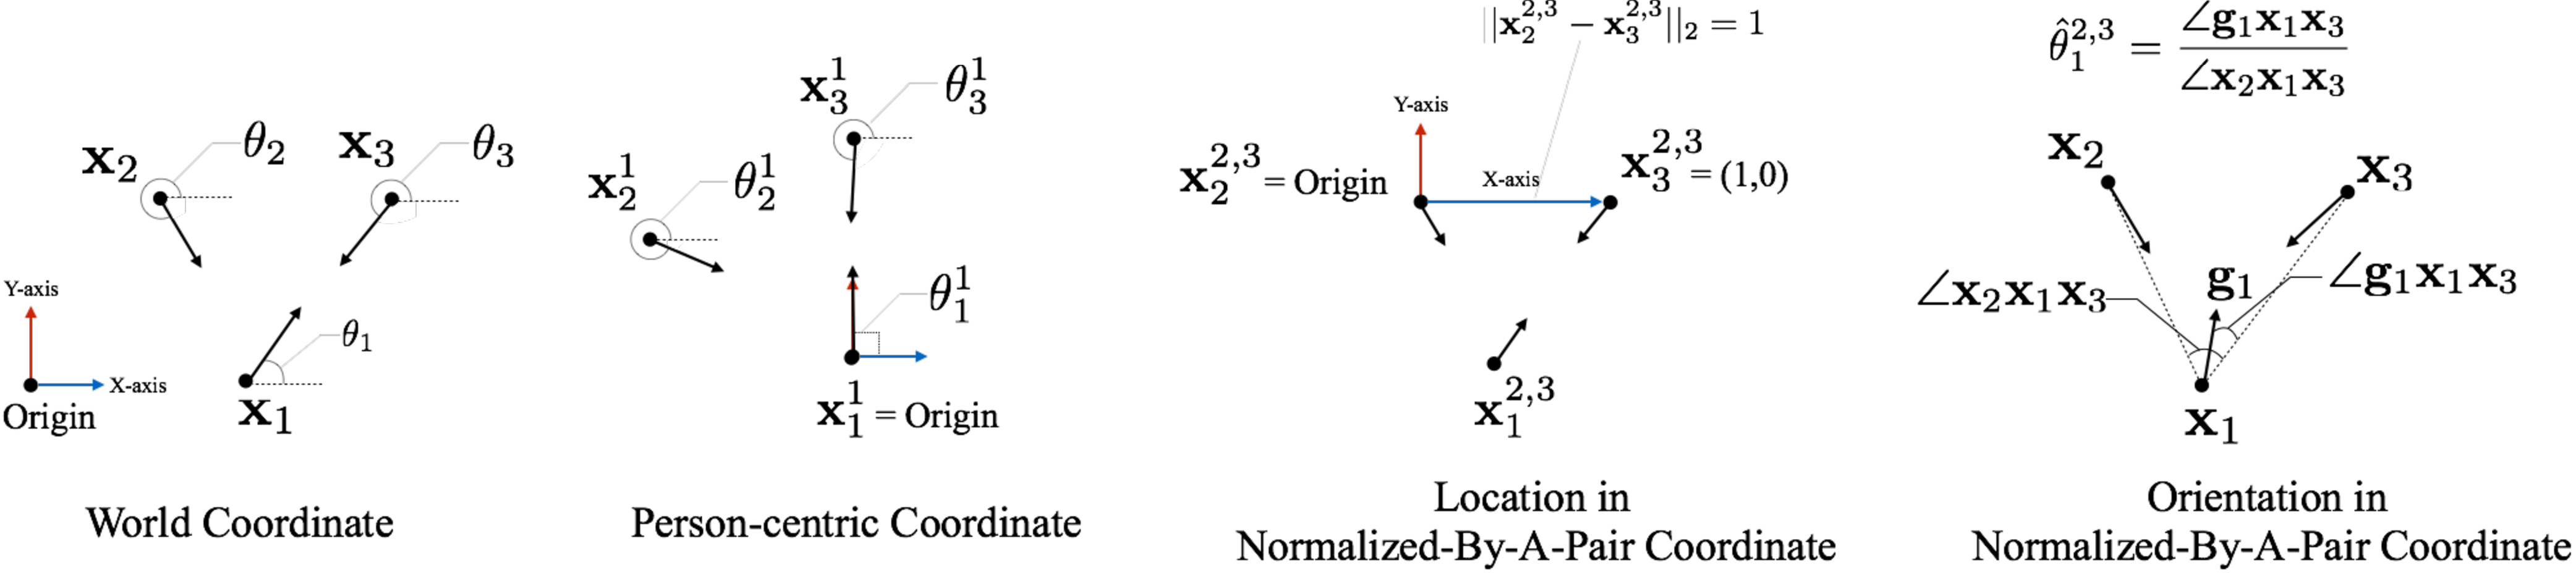
\includegraphics[width=\textwidth]{fig/ssp_notation3}
% 	\caption{Locations and orientations of an interacting group can be represented by different coordinate systems. (a) Locations and orientations in a world coordinate, (b) Locations and orientations in a person centric coordinate by person $\mathbf{P}_1$, (c) A location of $\mathbf{P}_1$  in a normalized coordinate by a pair of people $\mathbf{P}_2$ and $\mathbf{P}_3$, (d) An orientation of $\mathbf{P}_1$ in a normalized coordinate by a pair of people  $\mathbf{P}_2$ and $\mathbf{P}_3$. } 
% 	\label{fig:ssp_notation1}
% \end{figure*}

\subsection{Predicting Speaking}
\label{subsection:ssp_pred_speak}
As the first task, we predict whether the target subject is currently speaking or not. This is a binary classification task and relatively easier to train. We first study the correlation between the speaking signal and the target person's own social signals, either body motion or facial motion, or both. We expect this correlation is stronger than the link between individuals. We then compare it with the performance of a classifier that uses the conversational partner's social signals. More specifically, a function $\mathcal{F}_{j0\rightarrow s}$ uses the target person's own body motion $\mathbf{J}^0(t_0:t)$ to predict the speaking signal:
\begin{gather}	
\mathbf{S}^0(t_0:t) = \mathcal{F}_{J0\rightarrow S} \left( \mathbf{J}^0(t_0:t) \right),
\label{eq:speaking_0}
\end{gather}
and similarly,
\begin{gather}	
\mathbf{S}^0(t_0:t) = \mathcal{F}_{F0\rightarrow S} \left( \mathbf{F}^0(t_0:t) \right),\\
\mathbf{S}^0(t_0:t) = \mathcal{F}_{(F0, J0)\rightarrow S} \left( \mathbf{F}^0(t_0:t) , \mathbf{J}^0(t_0:t)\right),
\label{eq:speaking_0_facebody}
\end{gather}
where $\mathcal{F}_{F0\rightarrow S}$ uses the target person's own face motion, and $\mathcal{F}_{(F0, J0)\rightarrow S}$ uses both. 

We compare the performance of these functions with the functions that takes the signals from the communication partners:
\begin{gather}	
\mathbf{S}^0(t_0:t) = \mathcal{F}_{J12\rightarrow S} \left( \mathbf{J}^1(t_0:t), \mathbf{J}^2(t_0:t) \right),\\
\mathbf{S}^0(t_0:t) = \mathcal{F}_{F12\rightarrow S} \left( \mathbf{F}^1(t_0:t), \mathbf{F}^2(t_0:t) \right),\\
\mathbf{S}^0(t_0:t) = \mathcal{F}_{(F12, J12)\rightarrow S} \left( \mathbf{J}^1(t_0:t), \mathbf{J}^2(t_0:t), \mathbf{F}^1(t_0:t), \mathbf{F}^2(t_0:t) \right),
\label{eq:speaking_1}
\end{gather},
where the functions use body cues, face cues, and both cues, respectively. 

We hypothesize that the correlations of the target person's own signals are stronger than the correlations among the interpersonal signals, while we still expect that there exists a clear link in the latter case. We verify this in our experimental results.

%the social signals oindividual dynamics of the social signals is stronger than correlation between the speaking and the social signal body motion should be stronger than the speaking of the target and other people's body motions. But we still presume that there exists a clear correlation in building the function ~\ref{eq:speaking_1}; for example, if another person is talking we can guess the target person is not speaking due the ``turn-taking" implicitly followed during a social conversation. % This study is interesting because it demonstrates the existence of social correlation among social signals.

\paragraph{Implementation Details.}
\label{section:body2speak}
The input of this network is the body motion of the other seller in the haggling sequence, which is a $f \times 73$ matrix, where $f$ is the number of frames of an input sequence. Here, we ignore the buyer's body motion because often little movement is observed from the buyers.  We use four convolutional layers for the network where the last layer has $1\times1$ convolutions, followed by a sigmoid activation layer. The network architecture is shown in the first row of Figure~\ref{fig:architectures}.




\subsection{Predicting Social Formations}
As another sub-problem, we predict the location and orientations of the target person. This problem is strongly related to Proxemics~\cite{Hall66} and F-formation~\cite{kendon90}, illustrating how humans use their space in social communications.
\begin{gather}	
 \mathbf{Y}_p (t_0:t) = \mathcal{F}_p \left( \mathbf{X}_p^1(t_0:t), \mathbf{X}_p^2(t_0:t) \right),
 \label{eq:pred_formation}
\end{gather}
where $\mathbf{Y}_p$ and $\mathbf{X}_p^i$ contains global location and orientation signals $[\mathbf{x}, \boldsymbol{\theta}, \boldsymbol{\phi} ]$ for the target subject and others.
Note that we only consider the positions and orientations on the ground plane (in 2D), ignoring the height of the subjects. Thus $\mathbf{x} \in \mathbb{R}^2 $ representing $x$ and $z$ coordinate of the subjects. We use a 2D unit vector to represent the orientations $\theta \in \mathbb {R}^2$ and face orientation $\phi \in \mathbb{R}^2$, because the angle representation has a discontinuity issue when wrapping around $2\phi$ and $-2\phi$. In summary, $\mathbf{X}^i(t)$ and $\mathbf{X}^i(t)$ are a $6 \times N$ dimensional matrix where $N = t- t_0$ is the size of the temporal window. This prediction problem is intended to see whether the machine can learn how to build a social formation to interact with humans~\cite{vazquez2017towards}. %We Social formation is one of the most noticeable social properties with strong correlation, allowing us to easily evaluate the performance.


\paragraph{Implementation Details.}
We use a 2D vector for the position and 2D unit vectors for the face orientation and body orientation, defined on the $xz$-plane. Thus the status of an individual at a frame in social formation prediction is represented by a 6-dimensional vector.


The input of the social formation network is the concatenation of global position and orientation information of the communication partners, represented by a $f \times 12$ matrix.  We use a simple autoencoder structure, as shown in the second row of Figure~\ref{fig:architectures}.


%To implement this, we use a simple 1-D temporal convolutional neural network to model $\mathcal{F}_p$. The network is trained with a window of frames $N=120$ (corresponding to 4 seconds), but arbitrary length of input can be used in testing time since our network is fully convolutional. We use a simple encoder-decoder network. The encoder has  3 convolutional layers followed by dropout (0.25) and RELU, and 1D pooling layer (with stride 2). The decoder uses a single transposed convolution layer. We use L2 loss function with a L1 regularization term (with weight 0.1). We simply use the global position and orientations with standardization, rather than any local or relative coordinate.
